\begin{center}
    PRACTICA DE LABORATORIO N° 03
\end{center}

\section{Objetivos}
Crear relaciones automáticas y manuales

\section{Requerimientos}

\begin{itemize}

- Conocimientos básicos de administración de base de datos Microsoft   SQL Server.
\\- Conocimientos básicos de SQL.
\\- Microsoft SQL Server 2016 o superior
\\- Base de datos AdventureWorks2016 o superior
\\- Power BI Desktop.
\\- Tener una cuenta Microsoft registrada en el Portal de Power Bi.

\end{itemize}

\section{Desarrollo} 
\textbf{1. Conectar a datos existentes}

\begin{center}
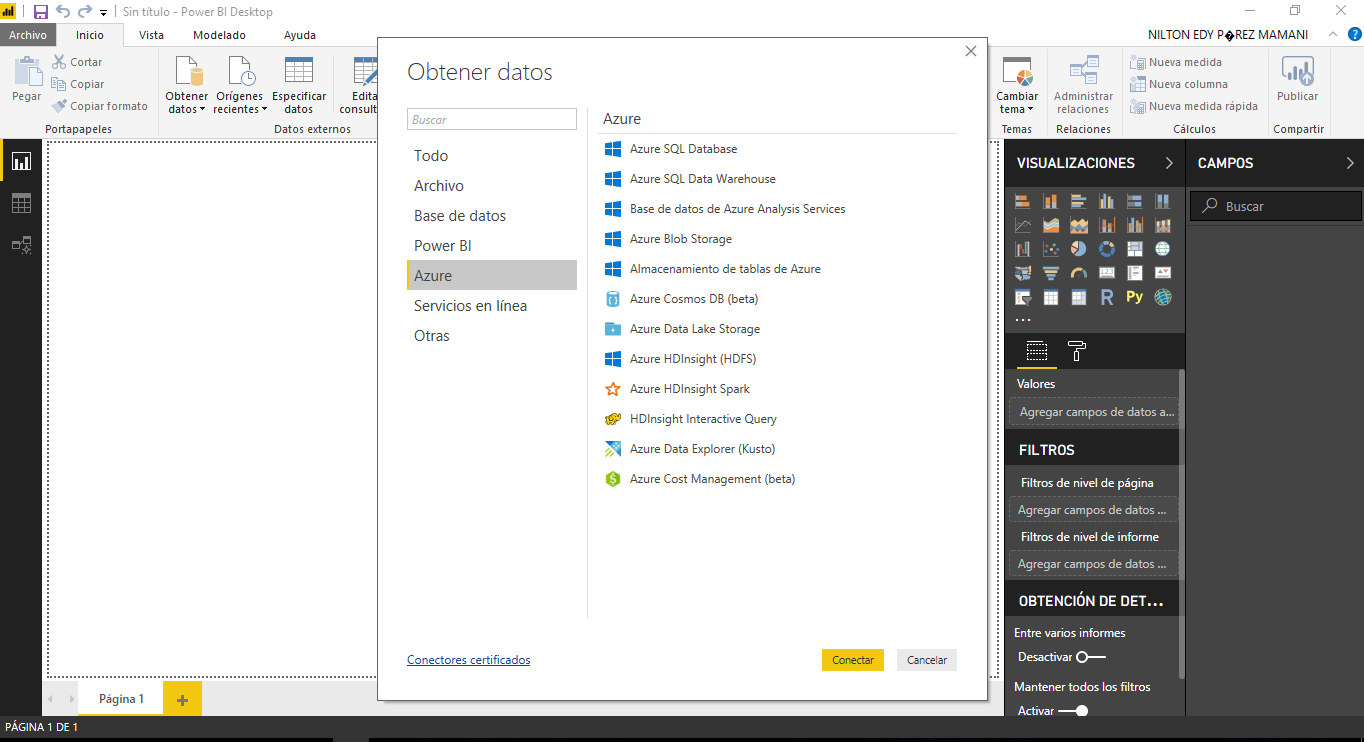
\includegraphics[width=15cm]{./Imagenes/imagen1}
\end{center}

\begin{center}
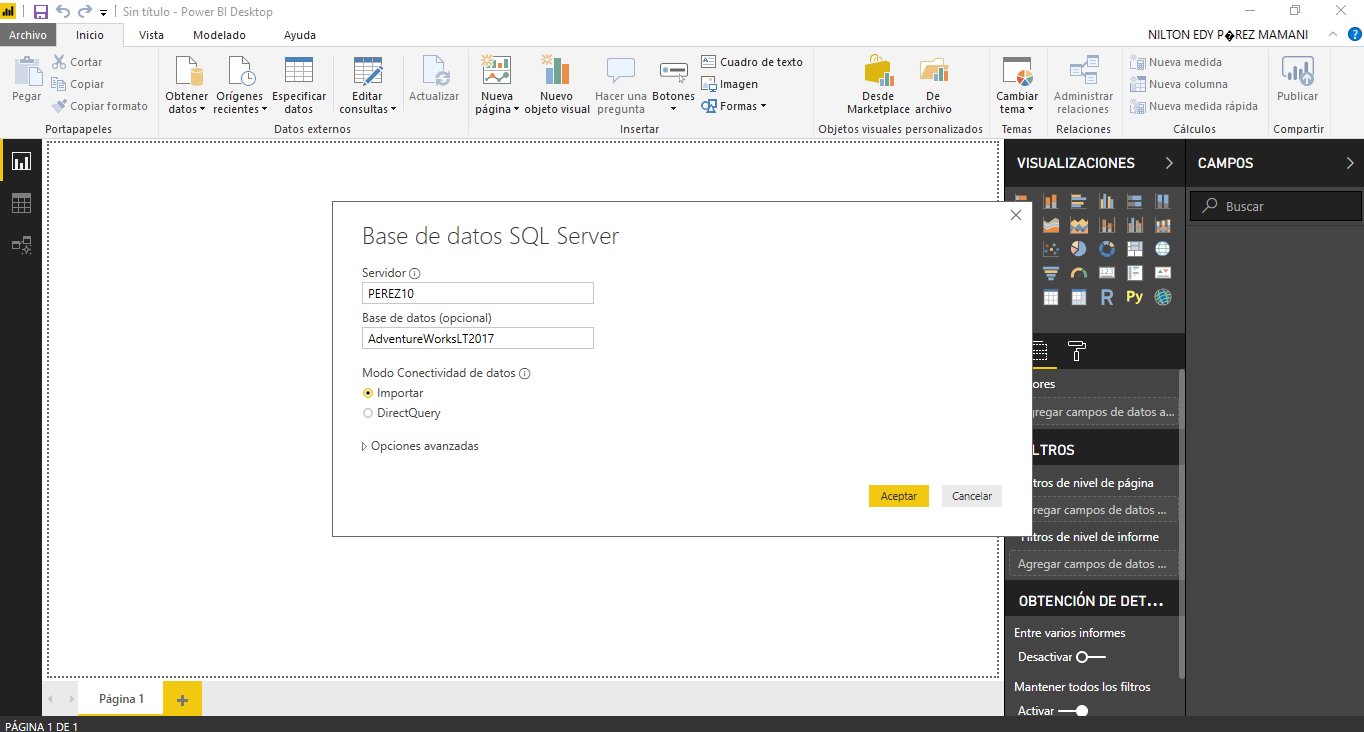
\includegraphics[width=15cm]{./Imagenes/imagen2}
\end{center}

\begin{center}
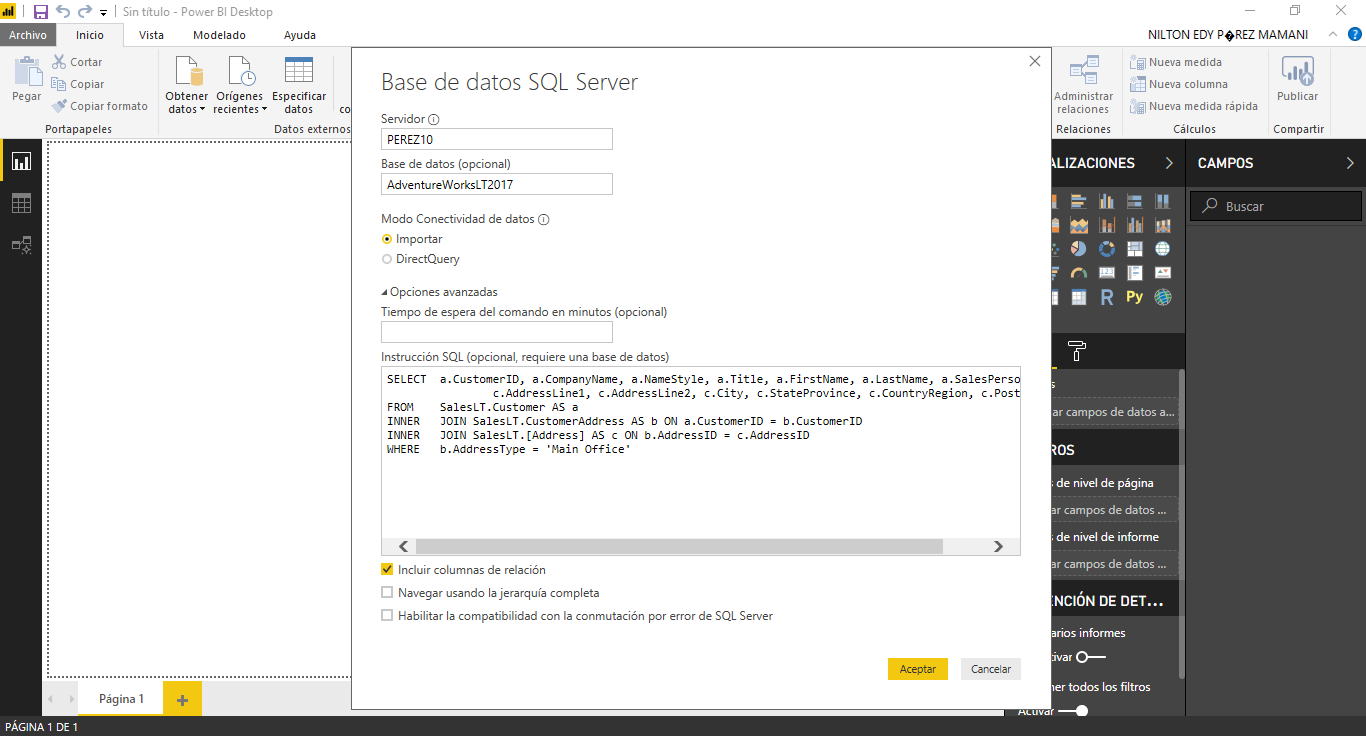
\includegraphics[width=15cm]{./Imagenes/imagen3}
\end{center}

\begin{center}
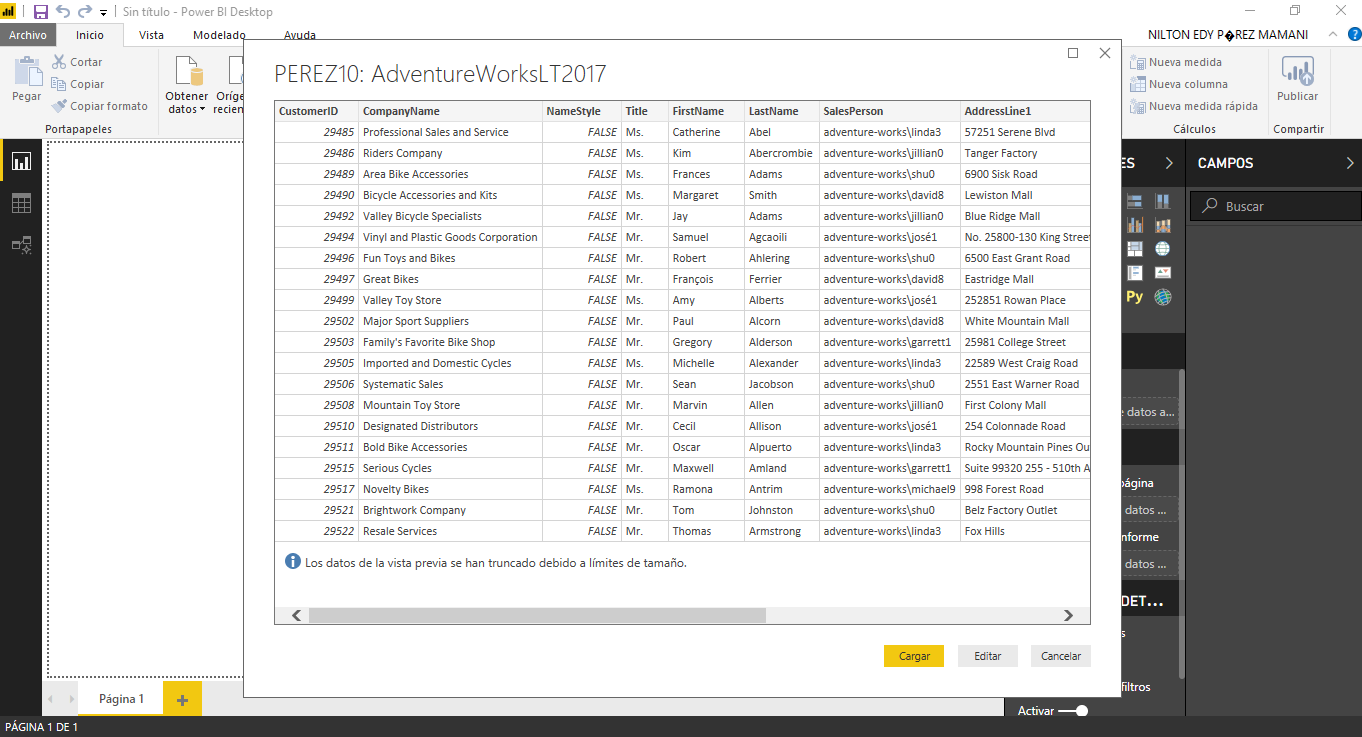
\includegraphics[width=15cm]{./Imagenes/imagen4}
\end{center}

\begin{center}
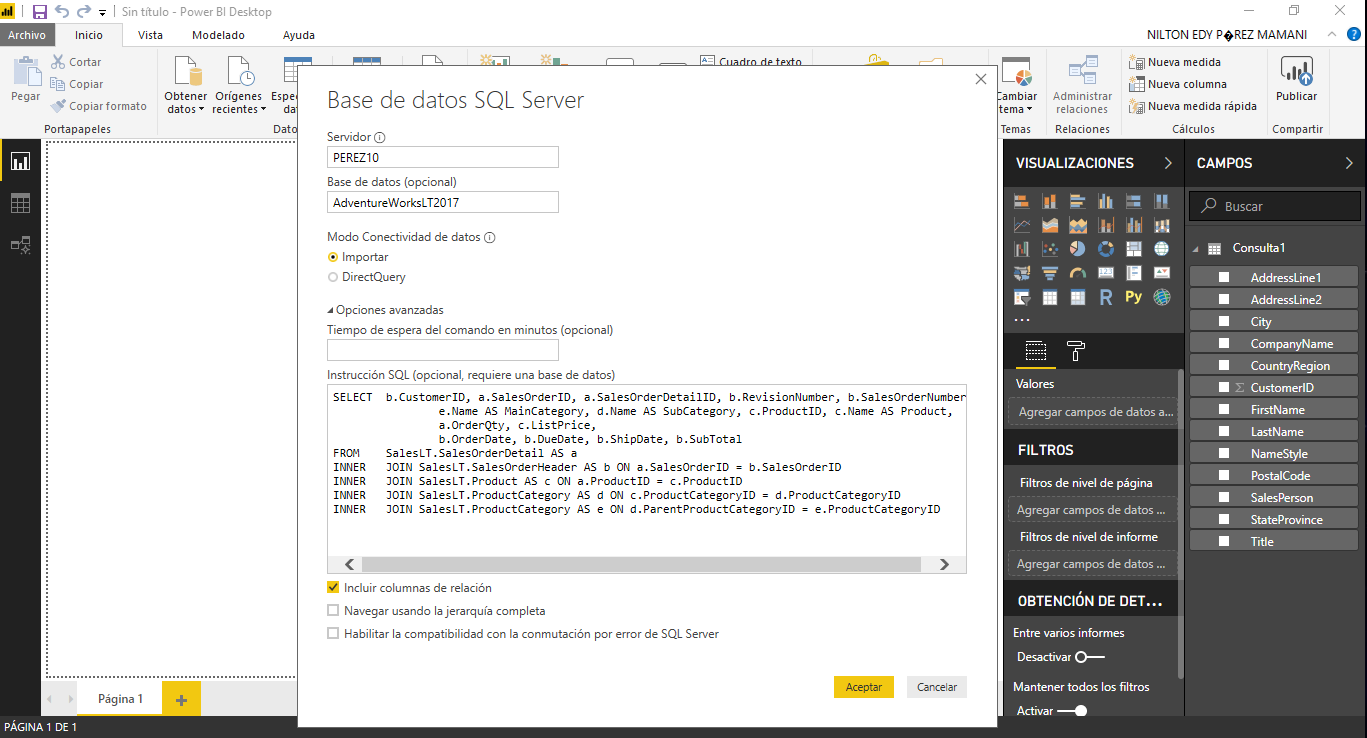
\includegraphics[width=15cm]{./Imagenes/imagen5}
\end{center}

\begin{center}
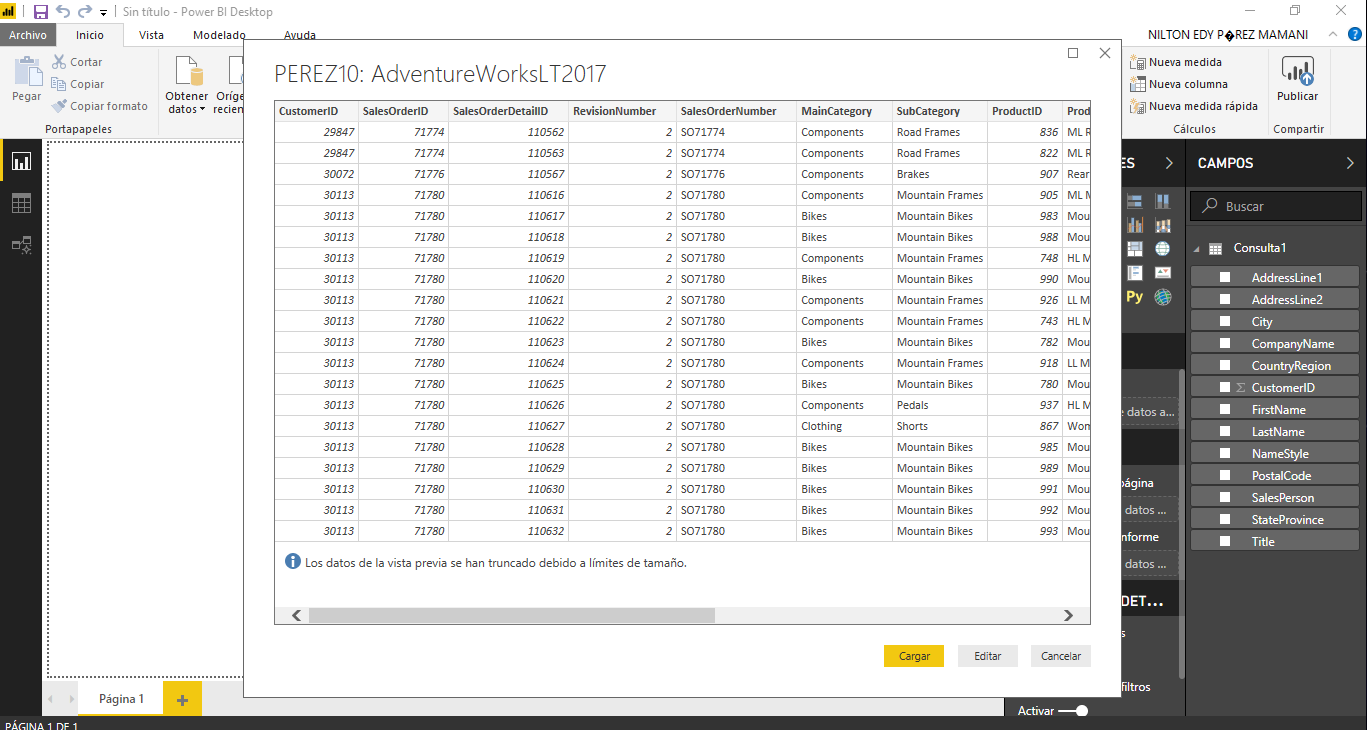
\includegraphics[width=15cm]{./Imagenes/imagen6}
\end{center}

\textbf{2.Datos de forma}

\begin{center}
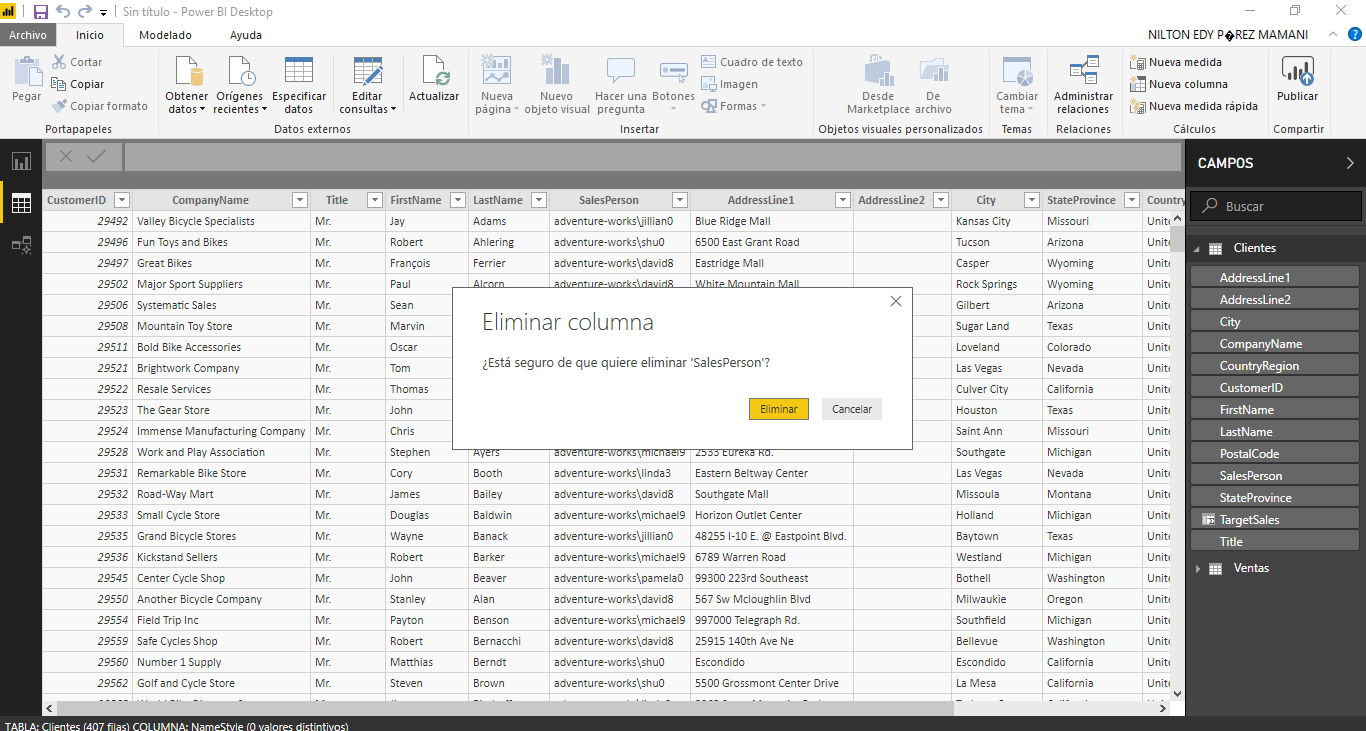
\includegraphics[width=15cm]{./Imagenes/imagen7}
\end{center}

\begin{center}
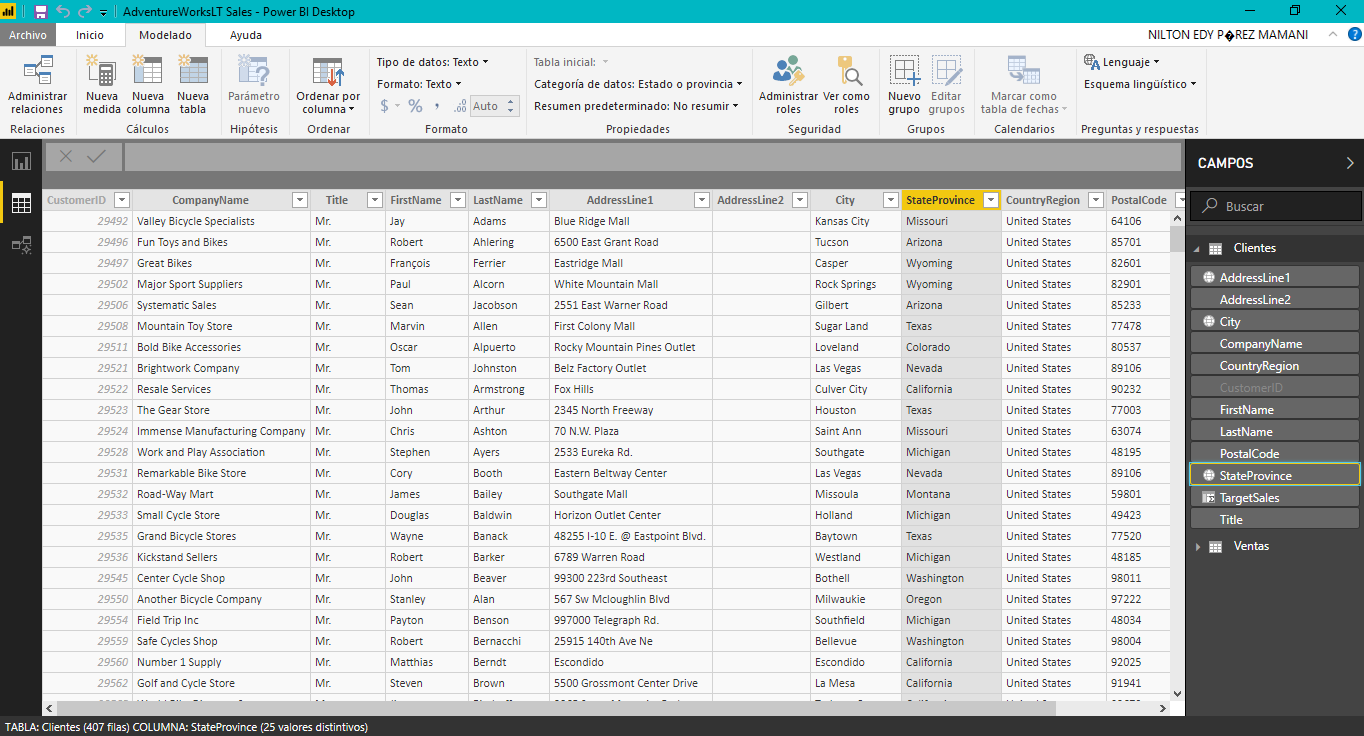
\includegraphics[width=15cm]{./Imagenes/imagen8}
\end{center}

\begin{center}
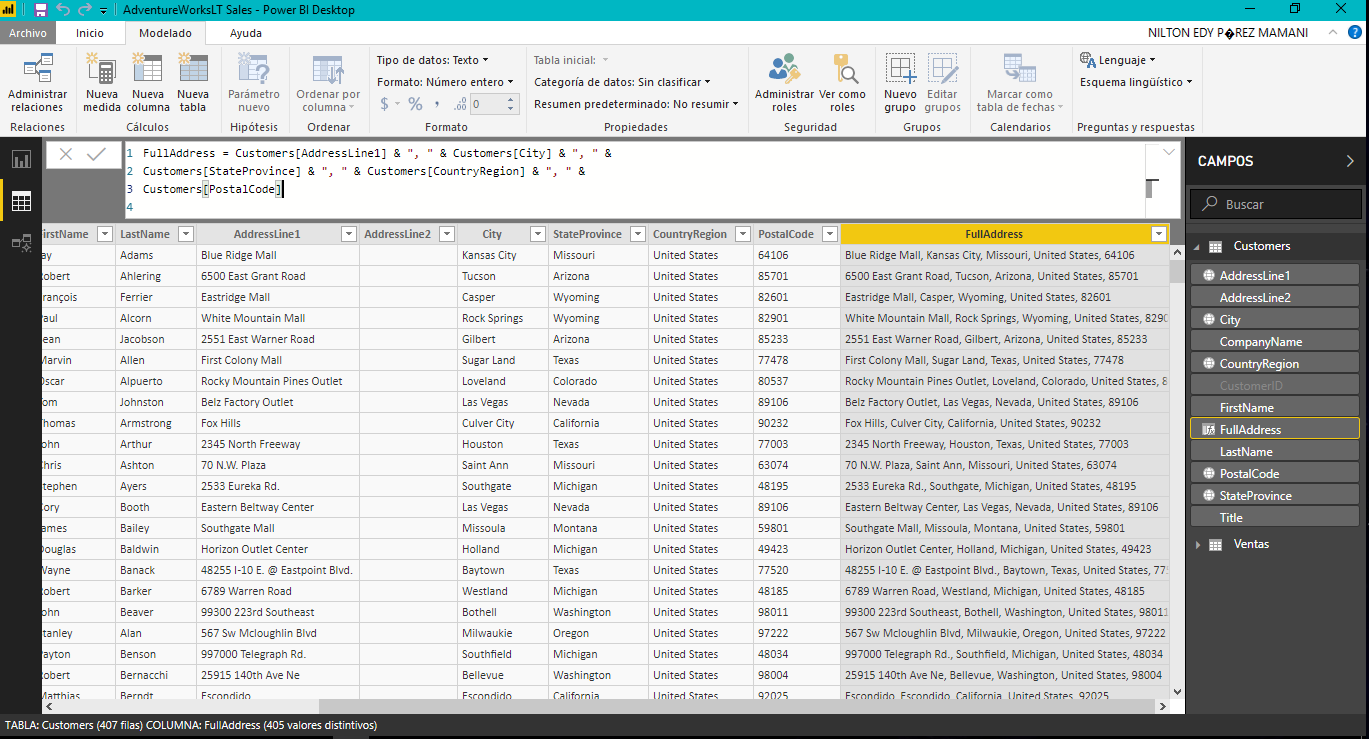
\includegraphics[width=15cm]{./Imagenes/imagen9}
\end{center}

\begin{center}
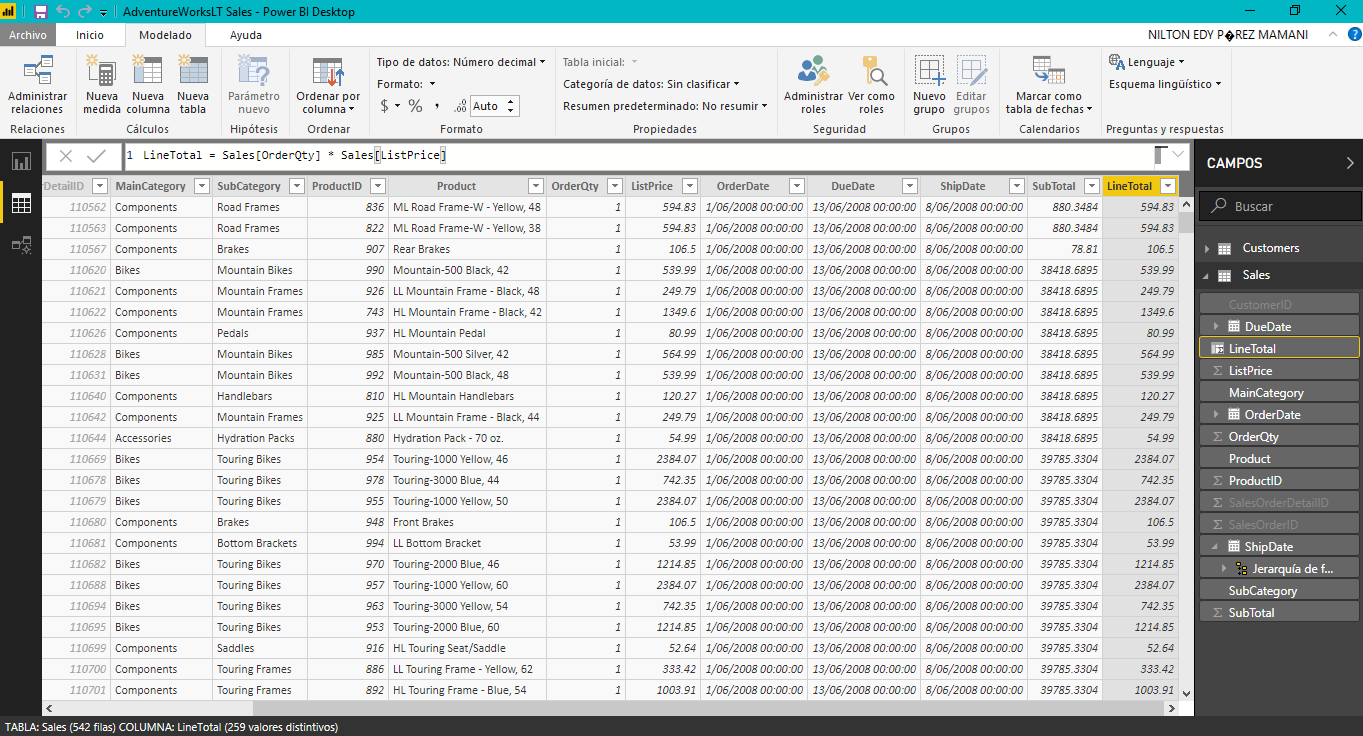
\includegraphics[width=15cm]{./Imagenes/imagen10}
\end{center}

\begin{center}
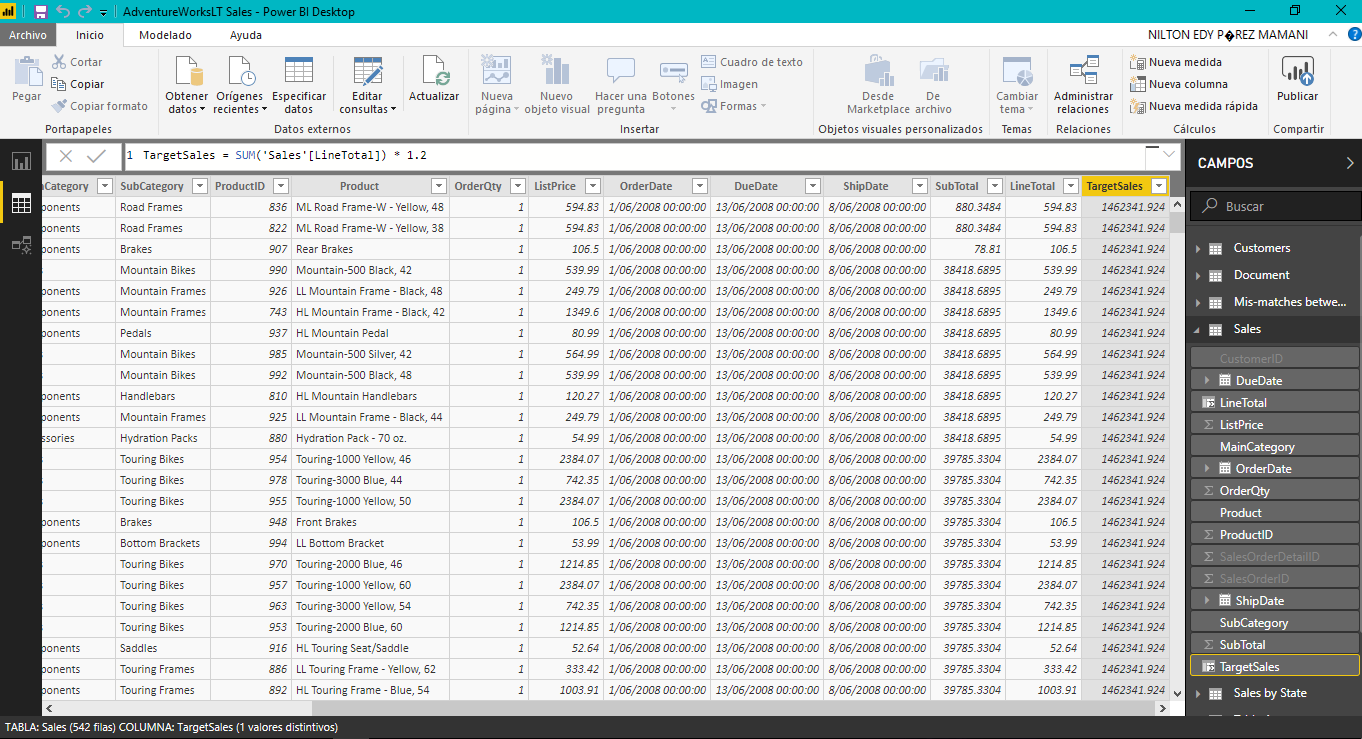
\includegraphics[width=15cm]{./Imagenes/imagen11}
\end{center}

\textbf{3.Crear un Gráfico}

\begin{center}
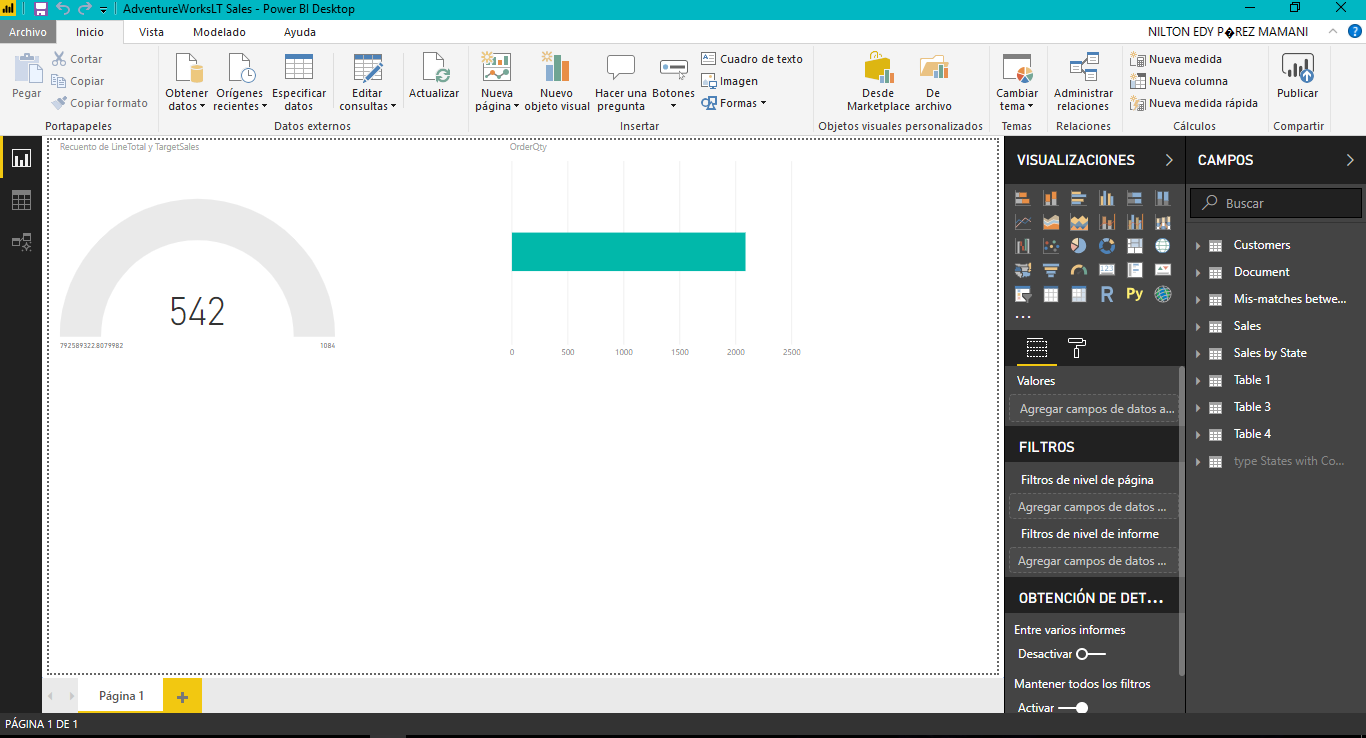
\includegraphics[width=15cm]{./Imagenes/imagen12}
\end{center}